\documentclass[12pt,a4paper,dvipdfmx]{jarticle}
\usepackage[top = 20truemm, bottom = 20truemm, left = 15truemm , right = 15truemm]{geometry}
\usepackage[dvipdfmx]{graphicx}
\usepackage{here}
\usepackage[dvipdfmx]{hyperref}
\usepackage{pxjahyper}
\hypersetup{
	bookmarksnumbered = true,
	colorlinks = true,
	setpagesize = false,
	linkcolor = blue,
	urlcolor = blue
}
\title{モータシステム:スナバ回路設計データ}
\author{小野澤颯}
\begin{document}
\maketitle
\section {目次}
\begin {enumerate}
	\item \hyperlink{section1}{スナバ回路について}
	\item \hyperlink{section2}{非放電型スナバ回路の計算}
	\item \hyperlink{section3}{モータシステムFETブリッジへの実装}
	\item \hyperlink{section4}{参考文献}
\end{enumerate}
\section {本編}
\begin{enumerate}
	\item \hypertarget{section1}{スナバ回路について}\\
		 MOSFETは非常に高速でスイッチングされるため、ドレイン電流の変化は非常に急となる。例えば、モータ制御回路のHブリッジ部に注目し、ハイサイドFETがターンオンしているときモータに電流$I$が流れる。次にターンオフしたとき、配線の寄生インダクタンス$L_{parasitic}$、モータのインダクタンス成分$L_{m}$によって、ドレインソース間には$(L_{parasitic}+L_{m})\frac{dI}{dt}$に従い、大きなサージ電圧が発生する。このサージ電圧がFETの$V_{ds(max)}$を超えると破壊原因となる。\\
		\begin{figure}[H]
		\centering
		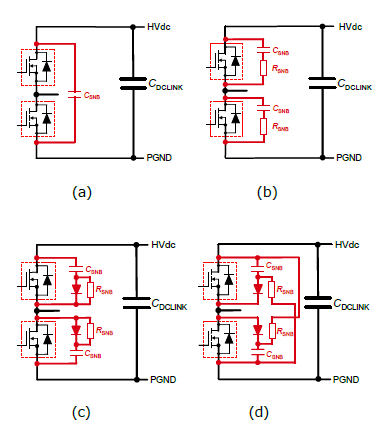
\includegraphics[width=6cm]{snb.jpg}
		\caption{各種スナバ回路}
		\end{figure}
		 スナバ回路は破壊原因となる寄生成分にサージを吸収し、FETの過渡電圧保護する保護回路である。スナバ回路には大きく4種類あり、まず図1.(a)のCスナバ回路、次に図1.(b)に示すRCスナバ回路、図1.(c)のRCDスナバ回路、図1.(d)の非放電型RCDスナバ回路である。ここでは、非放電型RCDスナバ回路を取り扱う。\\
		 非放電型RCDスナバ回路は各種スナバ回路の中でもっともサージ吸収効果の高めることが可能な回路であり、スナバコンデンサのスイッチング毎の放電が行われないため、スナバ抵抗の消費電力はサージによる電力のみとなり、スナバコンデンサの値を大きくすることができ、サージ吸収効果を大きく高めることが可能となる。他のスナバ回路ではスナバコンデンサがスイッチング毎に放電し、スナバ抵抗で電力を消費するため、スナバコンデンサの大きさが制限されてしまう。しかし、非放電型スナバ回路はもっとも配線レイアウトが複雑になり、層の少ない基板では実装するのが困難である。
	\item \hypertarget{section2}{非放電型RCDスナバ回路の計算}\\
		  非放電型RCDスナバ回路の設計方法を示します。寄生インダクタンスにたまったエネルギーをスナバコンデンサで吸収することでサージを吸収しているため、スナバコンデンサは
		 \begin{equation}
		 \label{csnb}
		 C_{snb}>\frac{L_{parasitic}I^2}{(V_{ds(surge)}-V_{source})^2}
		 \end{equation}
		で求める。これはインダクタンスのエネルギー式とコンデンサのエネルギー式から明らかである。\\
		 次に、吸収した電力の90\%を消費するスナバ抵抗の設計方法を示す。
		\begin{equation}
		\label{rsnb}
		R_{snb}<\frac{1}{f_{sw}C_{snb}2.3}
		\end{equation}
		 この抵抗器は、小さすぎると発振する可能性があるためできるだけ用件満たす範囲で多き値を使う。\\
		 上式の求め方を下記に簡単に示す。前提として、$V_c=V_{source}(1-e^{-\frac{t}{rc}})$はRC直列回路のコンデンサ電位のt軸関数である。
		\begin{eqnarray}
		V_{c(snb)}=V_{ds(surge)}(1-e^{-\frac{t}{R_{snb}C_{snb}}})
		\end{eqnarray}
		tはスイッチング周期だから $t=\frac{1}{f_{sw}}$
		\begin{eqnarray}
		V_{c(snb)}=V_{ds(surge)}(1-e^{-\frac{1}{f_{sw}R_{snb}C_{snb}}})\\
		e^{-\frac{1}{f_{sw}R_{snb}C_{snb}}}=\frac{V_{ds(surge)}-V_{c(snb)}}{V_{ds(surge)}}\\
		-\frac{1}{f_{sw}R_{snb}C_{snb}}=log[\frac{V_{ds(surge)}-V_{c(snb)}}{V_{ds(surge)}}
]\\
		R_{snb}=\frac{-1}{f_{sw}C_{snb}log[\frac{V_{ds(surge)}-V_{c(snb)}}{V_{ds(surge)}}
]}
		\end{eqnarray}
		コンデンサ電位を90\%消費するとき $V_{c(snb)}=0.9V_{ds(surge)}$\\
		\begin{eqnarray}
		log[\frac{V_{ds(surge)}-0.9V_{ds(surge)}}{V_{ds(surge)}}]\simeq-2.3
		\end{eqnarray}
		 次に、スナバ抵抗の消費電力の設計方法を示す。\\
		\begin{equation}
		\label{psnb}
		P_{snb}=\frac{L_{parasitic}I^2f_sw}{2}
		\end{equation}
		 これは、寄生インダクタンスのエネルギーがスイッチング毎に消費されていることを示している。\\
	\item \hypertarget{section3}{モータシステムFETブリッジへの実装}\\
		 用いるスナバ回路はまず、モータシステムで扱う最大電流$I_{max}$、電源電圧$V_{source}$、FETの絶対最大定格$V_{max}$、PWM周波数$f_{sw}$を定義する。\\
		 例として、(あくまで例です(重要なことなので二回言います))
		\begin{eqnarray}
			I_{max} = 100 [A]\\
			V_{source} = 24 [V]\\
			V_{max} = 30 [V]\\
			f_{sw} = 100 [kHz]
		\end{eqnarray}
		と定義する。また、ここでは寄生インダクタンスを$100nH$と定義する。\\
		 したがって、式\ref{csnb}より、$C_{snb} > 0.28 [nF]$となり、E系列より$0.33[\mu F]$を選択する。\\
		  式\ref{rsnb}より、$R_{snb} < 13 [\Omega]$となるため、$10 [\Omega]$を選択する。\\
		  式\ref{psnb}より、抵抗の損失は$P_{snb} = 50[W]$となるが、この電力は現実的ではないため、100Aが流れる時はモータの過渡電流と考え、約0.1secとし、半分の$5[W]$抵抗を用いる。(これでもでかいなぁ)
	\item \hypertarget{section4}{参考文献}\\
		Rohm \href{https://fscdn.rohm.com/jp/products/databook/applinote/discrete/sic/mosfet/sic-mos_snubber_circuit_design_an-j.pdf}{アプリケーションノート[スナバ回路の設計](62AN036J)}\\
		富士電機 \href{https://www.fujielectric.co.jp/products/semiconductor/model/igbt/application/igbt.html}{アプリケーションノート[保護回路設計法]}
		
\end{enumerate}

\end{document}